\section{Experiments}\label{sec:experiments}

We evaluate the layer along four axes: the behaviour of the gradient at a synthetic branch crossing, the accuracy of the Laplace approximation against exact quadrature, the algebraic and relaxation results, and a real two-mode cost assembled from LINEMOD depth. All runs are CPU-only, single-process jobs.

\subsection{Setup and metrics}\label{sec:metrics}

We evaluate on an 81-point synthetic crossing grid over $[-0.2,0.2]$ and on 15 real LINEMOD frames (8 \texttt{eggbox}, 7 \texttt{glue}). The synthetic benchmark returns all local minima together with a branch-following finite-difference (FD) reference; the 1D normal forms are the only setting in which the posterior integral is computed by dense quadrature. The synthetic instance is constructed, not fitted: $M(\theta)=M_{\rm sym}+\theta M_{\rm break}$ with a $P$-invariant double well, $d(J_B-J_A)/d\theta|_{\theta=0}=2.0$, a fixed translation block with $G\succ0$, and seed 20261127; enumeration is a batched damped Newton on $\mathbb{S}^3$ with 128 random starts, $SO(3)$-distance deduplication ($10^{-5}$ rad) and a stationarity filter ($\|\nabla J\|\le10^{-8}$, $\lambda_{\min}(H_{\mathbb{S}^3})>10^{-8}$). The real instance back-projects depth pixels inside the BOP \texttt{mask\_visib} with the real intrinsics, assigns each its nearest mesh vertex (KD-tree), and selects the dominant planar face by deterministic RANSAC (2.5 mm inlier band), with $n_{\rm points}=900$, $n_{\rm starts}=384$, $\tau=0.01$ and FD $h=10^{-4}$.

\textbf{Gradient relative error.} $\|\hat d\phi-d\phi_{\mathrm{FD}}\|_2/\|d\phi_{\mathrm{FD}}\|_2$ with $\phi=[\mathrm{vec}\,R(q);t^\star(q)]\in\mathbb{R}^{12}$, against a branch-following central FD ($h=10^{-4}$ for Parts A and B, $h=10^{-3}$ otherwise; the timing study uses a Richardson-extrapolated reference). For the hard argmin at a global tie the reference branch switches inside $\pm h$ and the entry is N/A; the FD truncation is measured separately.

\textbf{MC pose spread.} Euclidean norm of the standard deviation of $\phi$ over 20 independent mode-level MC means, each from $n=200$ samples; the translation block is fixed at $D_{\text{scale}}=0.30$, so this is a relative spread. Part B uses $n=400$ per $\theta$; the timing study uses $n=200$ with 3 seeds.

\textbf{Pose error, ADD-S and ADD.} Rotation error is $\arccos((\operatorname{tr}(R_{\rm est}^\top R_{\rm gt})-1)/2)$ in degrees on a proper rotation; translation error is $\|t_{\rm est}-t_{\rm gt}\|$ in metres (BOP \texttt{cam\_t\_m2c} is in millimetres). The Laplace estimate is the \textbf{projected chordal mean} $R_{\rm Lap}=\mathrm{Proj}_{SO(3)}(\sum_kw_kR_k)$ with $t_{\rm Lap}=\sum_kw_kt_k$. The raw 9-vector average is not orthogonal, so the geodesic formula applied to it gives $58.28^\circ$ rather than a rotation error; on the projected mean the median is $44.24^\circ$, and ADD-S is defined only for the projected pose. ADD-S transforms 1000 query vertices and matches each to the nearest vertex of the GT-transformed \emph{full} mesh (18{,}473 \texttt{eggbox} / 7{,}479 \texttt{glue} vertices; three query subsamples): $\mathrm{ADD\text{-}S}=\frac{1}{|V|}\sum_{x\in V}\min_{y\in V_{\rm gt}}\|R_{\rm est}x+t_{\rm est}-(R_{\rm gt}y+t_{\rm gt})\|$. The 1000-vertex GT variant carries a $+1.1$ mm discretisation floor (hard pose), while the dense-GT estimator agrees with full-mesh-vs-full-mesh ADD-S to $0.51$ mm. ADD uses the same-index distance and is reported only as a reference; ADD-S is appropriate because \texttt{eggbox} (obj 10) and \texttt{glue} (obj 11) each have a discrete $\sim180^\circ$ symmetry, and ADD would charge a symmetry-equivalent pose an error of order the object diameter ($0.165$ m / $0.176$ m).

\textbf{CIs, bias and derived quantities.} Percentile bootstrap over frames (1000 resamples for pose error, 2000 for the classical solvers); the paired bias is the mean per-frame difference against the hard argmin. With 15 frames the CIs describe this fixed set, not a population; for MC, a seed-level bootstrap over the 20 per-seed aggregates isolates seed noise (between-seed SD of the aggregate rotation error $1.011^\circ$). Wall-clock is CPU milliseconds per layer call (20-repetition medians and p95). The 1D error is $|E_{\mathrm{Lap}}-E_{\mathrm{exact}}|$, its ratio to $\tau$, the log-log slope versus $\tau$ and the relative gradient error; the fold error is $|Z_{\mathrm{Lap}}-Z_{\mathrm{exact}}|/Z_{\mathrm{exact}}$. SDP quantities are the primal value, dual $\mu$, $\lambda_{\min}(Z)$, $\operatorname{rank}(X^\star)$ at $10^{-6}$, $\lambda_1/\lambda_2$, the gap $f^\star-\mu$ and the exact constraint-span ranks (21 $\to$ 20; upstream 24 $\to$ 17; 24 + 3 row-orthogonality $\to$ 20). Derivative checks are relative errors of the Riemannian Hessian, the implicit Jacobians and $\partial_\theta\log\det H$ against central FD.

\subsection{Synthetic 6D branch crossing}\label{sec:synthetic}

Figure~\ref{fig:p1summary} summarises the four result families of this paper in one view: the 6D crossing, the measured 6D fold, the real LINEMOD two-mode structure, and the $10\times10$/$13\times13$ separation.

\begin{figure*}[t]
\centering
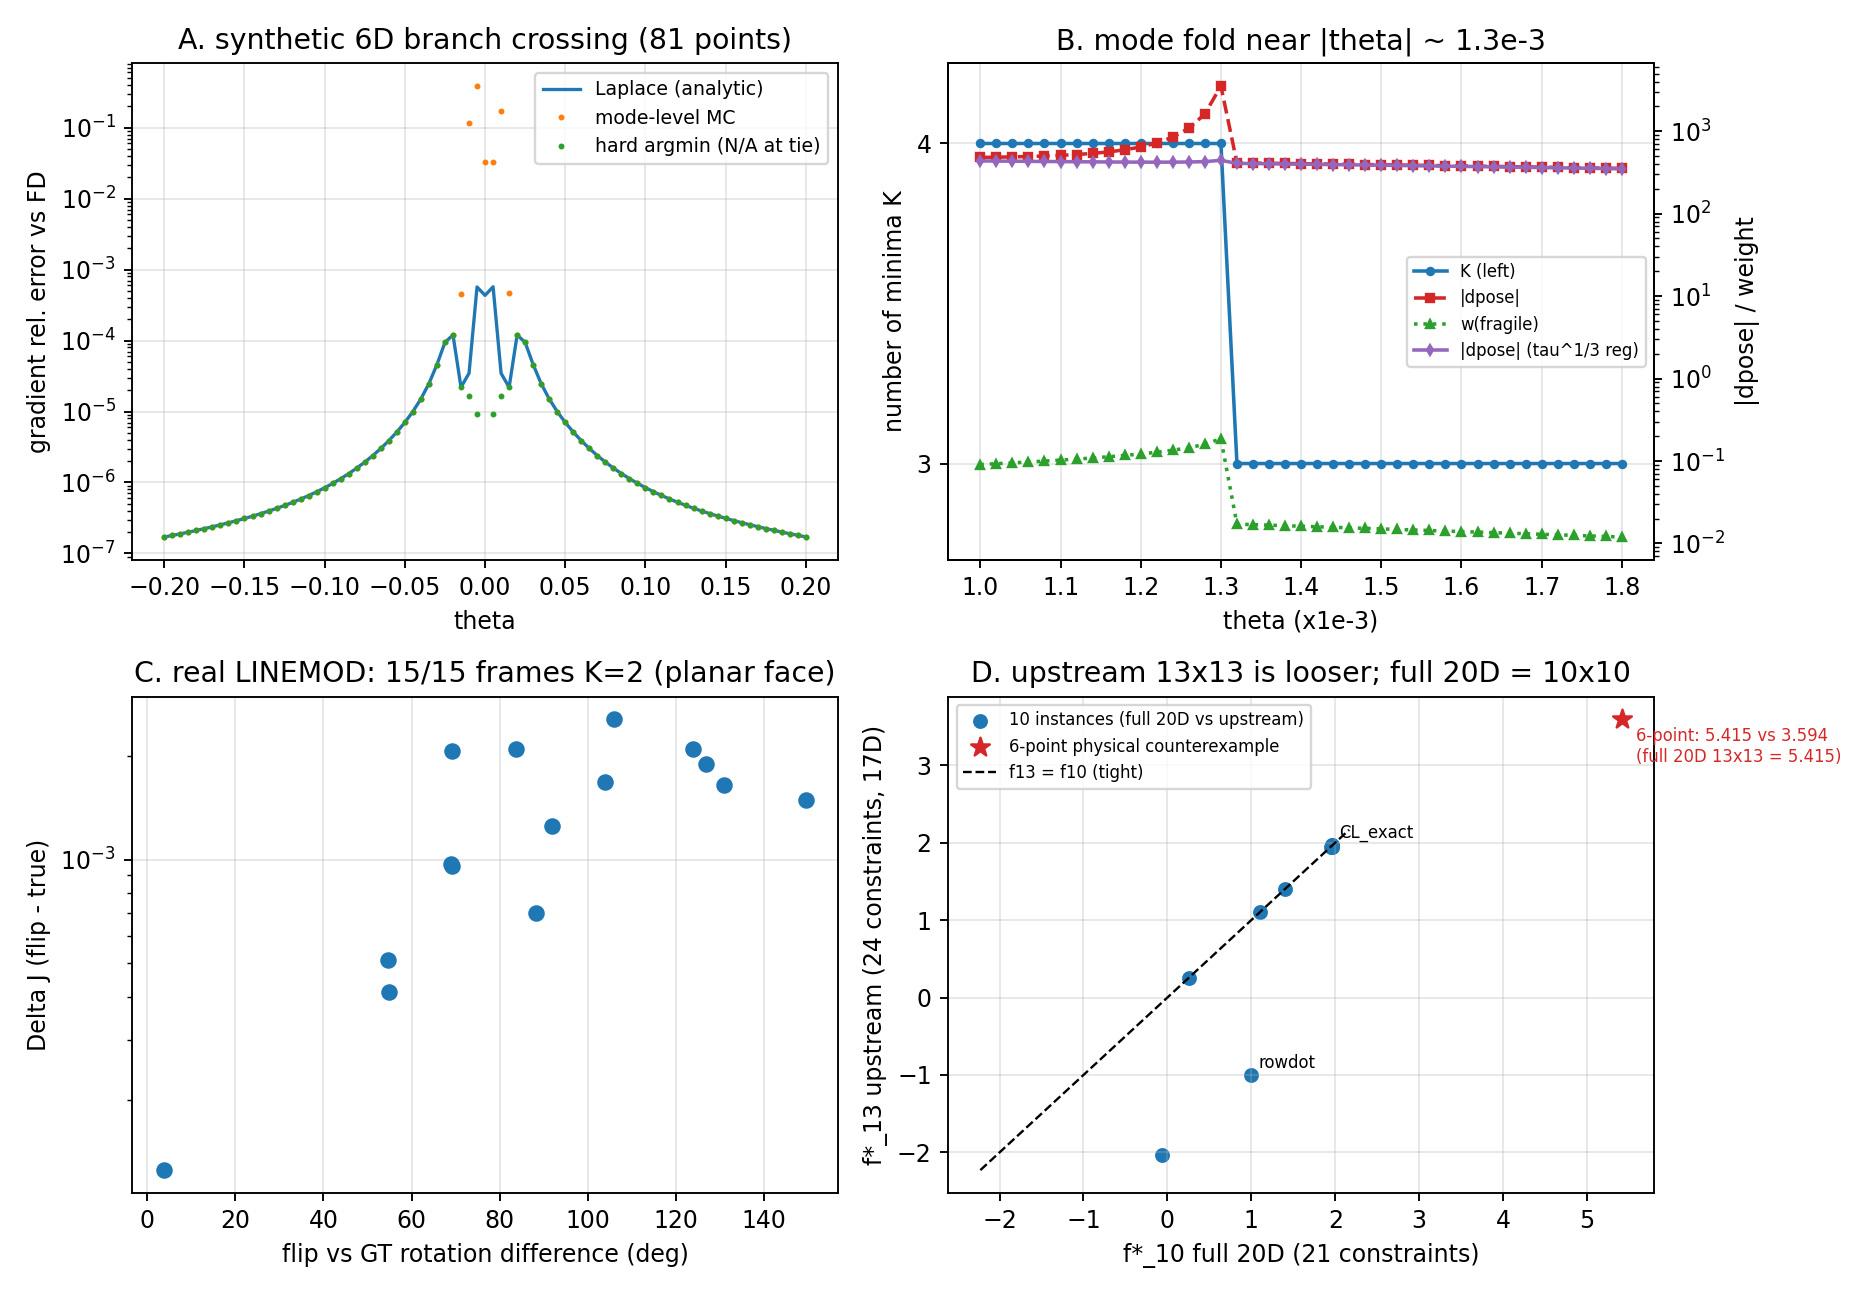
\includegraphics[width=0.92\textwidth]{p1_summary.png}
\caption{Overview of the four result families. \textbf{(A)} Gradient relative error vs $\theta$ on the 81-point synthetic 6D crossing for the analytic Laplace layer, the mode-level MC estimator and the hard argmin (N/A at the crossing); the Laplace curve has no jump, the hard map does. \textbf{(B)} The measured 6D fold near $|\theta|\sim1.3\times10^{-3}$: number of minima $K$, the pose-map jump $\|d\phi\|$ (standard and $\tau^{1/3}$-regularised) and the fragile-mode Laplace weight, all against $\theta$ on a $1.3\times10^{-3}$-scale axis; the mode dies at $\theta_f$ and $\|d\phi\|$ spikes there. \textbf{(C)} Real LINEMOD frames: the objective gap $\Delta J$ (flip minus true mode) against the flip-vs-GT rotation difference; all 15 frames have $K=2$. \textbf{(D)} Upstream 24-constraint $13\times13$ value against the full-20D $10\times10$ value on the 10 SDP instances and the 8 perturbations, with the six-point physical counterexample (star) separating the two: $5.415$ (full 20D) versus $3.594$ (upstream).}
\label{fig:p1summary}
\end{figure*}

\begin{table}[t]
\centering
\caption{Gradient relative error of the analytic Laplace layer, the mode-level MC baseline and the hard argmin, and the MC pose spread, per regime of the 81-point crossing grid ($\tau=0.01$, FD $h=10^{-4}$, mode-level MC $n=200$ with 20 seeds, CPU). Each entry is the median over the regime's grid points. The hard entry at $\theta=0$ is N/A because the global branch switches within $\pm h$.}
\label{tab:main6d}
\footnotesize
\setlength{\tabcolsep}{4pt}
\begin{tabular}{@{}l r l l l l@{}}
\toprule
regime & $n$ & Laplace & MC & hard & MC std\\
\midrule
far & 61 & 4.74e-07 & 4.74e-07 & 4.74e-07 & 2.76e-16\\
near & 19 & 3.46e-05 & 9.40e-05 & 2.23e-05 & 2.89e-16\\
at & 1 & 4.34e-04 & 3.26e-02 & N/A & 1.07e-01\\
\bottomrule
\end{tabular}
\end{table}

The grid has 61 far points, 19 near points and the single crossing point (nominal boundaries $|\theta|=0.05$ and $0.005$). Three observations follow.

\begin{enumerate}
\item \textbf{Away from the crossing the three methods coincide.} In the far regime all three median relative errors are $4.74\times10^{-7}$ and the median MC pose spread is $2.76\times10^{-16}$: the global mode carries essentially all of the Laplace mass and the sampler sees a single mode.
\item \textbf{The Laplace advantage is specific to the crossing.} In the near regime the hard argmin is still defined and has the smallest median error ($2.23\times10^{-5}$), ahead of Laplace and MC; the median MC spread is $2.89\times10^{-16}$, although the per-point maximum is $3.41\times10^{-2}$. At $\theta=0$ the hard entry is N/A, the Laplace entry is FD-limited (see below), and the MC error is $3.26\times10^{-2}$ with a pose spread of $1.07\times10^{-1}$.
\end{enumerate}

\textbf{The $4.34\times10^{-4}$ entry is FD truncation, not method error.} Against a Richardson-extrapolated FD it is $1.8\times10^{-7}$ at $\theta=0$, while against the plain central FD at $h=10^{-4}$ it is $4.3\times10^{-4}$; the sequence $4.34\times10^{-8}$ ($h=10^{-6}$), $4.34\times10^{-6}$ ($h=10^{-5}$), $4.34\times10^{-4}$ ($h=10^{-4}$) makes the same point. The near row is FD-limited for the same reason: at $\theta=0.01$ the study gives $3.46\times10^{-9}$ at $h=10^{-6}$ versus $3.46\times10^{-5}$ at $h=10^{-4}$. For $|\theta|\ge0.05$ the $h=10^{-5}$ error is at most $7.0\times10^{-8}$. The analytic gradient agrees with a Richardson FD to $1.8\times10^{-7}$ at the crossing, not to $4\times10^{-4}$.

\textbf{The hard argmin is a step map; the Laplace map is not.} The hard pose jump across $\theta=0$ stays $2.86$ as $\delta\to0$ ($\delta=10^{-3},10^{-4},10^{-5}$), while the Laplace jump decays linearly ($9.73\times10^{-1}$, $1.00\times10^{-1}$, $1.00\times10^{-2}$) with FD slope $\approx502$, i.e.\ the true derivative. Where its central FD is defined, the hard map is as self-consistent as Laplace (median $1.2\times10^{-4}$ over the non-switching cases), but it switches branch inside $\pm h$ in half of the exact-crossing cases. Fig.~\ref{fig:maintable} shows the per-point error and the MC spread.

\begin{figure}[t]
\centering
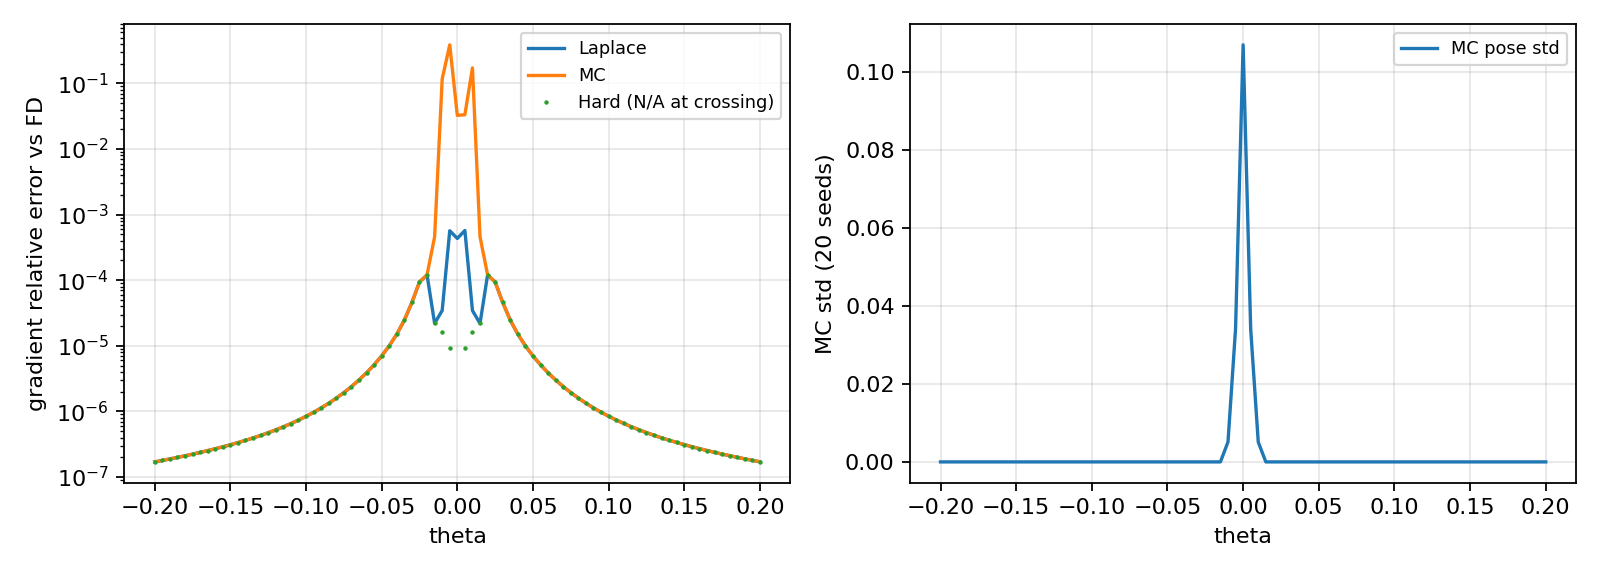
\includegraphics[width=\columnwidth]{main_table.png}
\caption{Main-table diagnostic on the 81-point 6D crossing grid. Left: gradient relative error against branch-following FD for the analytic Laplace layer (blue), the mode-level MC estimator (orange) and the hard argmin (green points; N/A at the exact crossing where the FD reference changes branch). Right: MC pose standard deviation over 20 seeds, which is essentially zero except in a narrow window around $\theta=0$.}
\label{fig:maintable}
\end{figure}

\textbf{The MC baseline is unbiased but noisy at a fixed budget.} On the same smoothed target, $n=200\times3$ seeds give a median per-seed gradient relative error of $0.05$ (20-seed mean $7.7\times10^{-3}$) and a median pose standard deviation of $0.09$ across the robustness conditions, versus $9.3\times10^{-8}$ for the analytic Laplace gradient against the Richardson reference. This is the measured variance cost of mode-level sampling.

\textbf{Mode count and fold.} The mode count over the grid is $K\in\{1,2,3,4\}$ ($K=1$ at 30 points, $K=2$ at 38, $K=3$ at 12, $K=4$ at the crossing point); these are the local minima returned by multi-start Newton with the filter above, not a certified root count. The smoothness statement is restricted to $\theta=0$ and $|\theta|\lesssim1.3\times10^{-3}$: a secondary minimum exists only there and disappears at the fold, where the Laplace map is discontinuous (Section~\ref{sec:fold6d}).

\subsection{1D exact posterior: the Laplace error is \texorpdfstring{$O(\tau)$}{O(tau)}}\label{sec:onepd}

\begin{table*}[t]
\centering
\caption{Exact posterior vs two-mode Laplace in the 1D normal form with unequal curvatures ($c=0.25$; at $g=0$ both minima sit at $x=\pm1$ with curvatures 5 and 3). $E$ is the posterior mean of $x$; errors are against a 2{,}000{,}001-point trapezoid on $[-3,3]$. Energies are dimensionless, and $\Delta J=6.16\times10^{-32}$ is numerical zero.}
\label{tab:1d}
\footnotesize
\setlength{\tabcolsep}{5pt}
\begin{tabular}{@{}l l l l l l l l@{}}
\toprule
regime & $\tau$ & $\Delta J$ & $E_{\mathrm{exact}}$ & $E_{\mathrm{Lap}}$ & $|{\rm err}|$ & $|{\rm err}|/\tau$ & rel grad err\\
\midrule
crossing & 0.05 & 6.16e-32 & -0.125102 & -0.127017 & 1.92e-03 & 3.83e-02 & 1.77e-02\\
crossing & 0.02 & 6.16e-32 & -0.126275 & -0.127017 & 7.42e-04 & 3.71e-02 & 6.93e-03\\
crossing & 0.01 & 6.16e-32 & -0.126649 & -0.127017 & 3.67e-04 & 3.67e-02 & 3.44e-03\\
crossing & 0.005 & 6.16e-32 & -0.126834 & -0.127017 & 1.83e-04 & 3.66e-02 & 1.71e-03\\
separated & 0.05 & 4.01e-01 & -1.024203 & -1.031750 & 7.55e-03 & 1.51e-01 & 2.77e-02\\
separated & 0.02 & 4.01e-01 & -1.029356 & -1.032296 & 2.94e-03 & 1.47e-01 & 1.27e-02\\
separated & 0.01 & 4.01e-01 & -1.030838 & -1.032296 & 1.46e-03 & 1.46e-01 & 6.27e-03\\
separated & 0.005 & 4.01e-01 & -1.031570 & -1.032296 & 7.26e-04 & 1.45e-01 & 3.12e-03\\
\bottomrule
\end{tabular}
\end{table*}

The expected-value error scales as $O(\tau)$: the log-log slope is 1.066 at the crossing and 1.036 in the separated basin, and $|{\rm err}|/\tau$ stays in $3.66$--$3.83\times10^{-2}$ at the crossing and $1.45$--$1.51\times10^{-1}$ when separated. The gradient error falls monotonically with $\tau$ on the printed rows; the gradient remainder is checked numerically rather than proved.

\subsection{Fold merging and the \texorpdfstring{$\tau^{1/3}$}{tau^(1/3)} regulariser}\label{sec:fold1d}

\begin{table*}[t]
\centering
\caption{Standard Laplace vs $\tau^{1/3}$-regularised volume factor at $\tau=0.01$, for $J=x^4/4-ax^2/2$; exact partition by a 2{,}000{,}001-point trapezoid on $[-3.5,3.5]$. $H=2a$ is the curvature at the minimum and the barrier is $a^2/4$.}
\label{tab:fold}
\scriptsize
\setlength{\tabcolsep}{2.5pt}
\begin{tabular}{@{}l l l l l l l l@{}}
\toprule
$a$ & $H$ & barrier & $Z_{\mathrm{exact}}$ & $Z_{\mathrm{Lap}}$ & rel err Lap & $Z_{\mathrm{reg}}$ & rel err reg\\
\midrule
0.50 & 1.00e+00 & 6.25e-02 & 2.6976e+02 & 2.5969e+02 & 3.73e-02 & 2.3556e+02 & 1.27e-01\\
0.20 & 4.00e-01 & 1.00e-02 & 2.3994e+00 & 2.1547e+00 & 1.02e-01 & 1.7371e+00 & 2.76e-01\\
0.10 & 2.00e-01 & 2.50e-03 & 1.2349e+00 & 1.4394e+00 & 1.66e-01 & 9.9871e-01 & 1.91e-01\\
0.05 & 1.00e-01 & 6.25e-04 & 9.7810e-01 & 1.6876e+00 & 7.25e-01 & 9.5017e-01 & 2.86e-02\\
0.02 & 4.00e-02 & 1.00e-04 & 8.6986e-01 & 2.5318e+00 & 1.91e+00 & 1.0019e+00 & 1.52e-01\\
0.01 & 2.00e-02 & 2.50e-05 & 8.3916e-01 & 3.5538e+00 & 3.24e+00 & 1.0358e+00 & 2.34e-01\\
\bottomrule
\end{tabular}
\end{table*}

As $a\to0$ the two minima and the saddle merge, $H\to0$, and the standard volume factor $1/\sqrt{H}$ diverges: the relative error grows from $3.73\times10^{-2}$ at $a=0.5$ to $1.91$ at $a=0.02$ and $3.24$ at $a=0.01$. Replacing $H$ by $H+\tau^{1/3}$ reduces the error to $1.52\times10^{-1}$ and $2.34\times10^{-1}$ at the two smallest $a$, but it is not uniformly better: at $a=0.5$ it is worse ($1.27\times10^{-1}$ versus $3.73\times10^{-2}$). The regularised form captures the $\tau^{1/3}$ scaling in the merging regime; it is not a drop-in replacement everywhere.

\subsubsection{The measured 6D fold}\label{sec:fold6d}

The 6D synthetic map has a genuine fold just off the crossing. A secondary minimum exists only for $|\theta|\lesssim1.3\times10^{-3}$ (the fine fold scan puts the mode death at $\theta_f=1.31\times10^{-3}$; the coarser robustness scan brackets it at $\approx1.4\times10^{-3}$); as it approaches the fold its $3\times3$ Hessian determinant falls through $3.35\times10^{-1}$ while its Laplace weight rises from $0.09$ to $0.187$ ($0.122$ at that determinant), and then the mode disappears ($K$ falls from 4 to 3). Across the fold the pose map steps by $0.31$ over one $2\times10^{-5}$ step (constant under grid refinement, i.e.\ a genuine discontinuity), and $\|d\phi\|$ peaks at $3529$ versus a median of $379$ away from the fold; the effective FD slope reaches $1.5\times10^4$. Neither a smaller $\tau$ nor more starts removes it: $n_{\rm starts}\ge32$ matches the 1024-start median $K$ (64 starts reproduce the full mode set on the sweep), while $n_{\rm starts}=16$ misses the fragile mode in 10\% of independent draws and a miss moves the pose by up to 28\% and the gradient by up to 97\%. The smoothness and $O(\tau)$ accuracy statements are therefore restricted to $\theta=0$ and $|\theta|\lesssim1.3\times10^{-3}$; the multi-modal Laplace map is discontinuous where a minimum is born or dies.

\textbf{A partial fix for the fold.} Replacing $\det H$ by $\det(H+\epsilon I)$ with $\epsilon=\tau^{1/3}$ (the 1D rule above, whose derivative is still closed form, $\operatorname{tr}((H+\epsilon I)^{-1}\dot H)$) largely removes the \emph{derivative} singularity: at $\theta=1.30\times10^{-3}$ the standard $\|d\phi\|$ is $3529$ while the regularised one is $443$, and the near-fold gradient error falls from $2.90\times10^{-1}$ to $1.19\times10^{-2}$ (a factor 24); away from the fold ($\theta=0.1,0.02$) the two variants agree to the printed precision. It does not remove the \emph{value} discontinuity caused by a minimum dying: the pose step across the fold only falls from $0.309$ to $0.107$ and $K$ still changes from 4 to 3. Hessian regularisation is therefore a cheap mitigation for the fold neighbourhood; a continuity claim across the fold requires the Scorer continuation of Section~\ref{sec:discussion} or a local numerical integral over the merging pair.

\subsection{Rotation-SDP certificate and the three-part \texorpdfstring{$10\times10$/$13\times13$}{10x10/13x13} relation}\label{sec:results_sdp}

\begin{table}[t]
\centering
\caption{Numerical certificate for the constructed $10\times10$ rotation SDP (Choi--Lam quartic plus $2I$; SCS). The gap is $f^\star-\mu$, where $f^\star=2$ is the analytic minimum of the quartic on $\mathbb{S}^3$ and $\mu$ is the certified dual value.}
\label{tab:sdp_cert}
\scriptsize
\setlength{\tabcolsep}{3pt}
\begin{tabular}{@{}p{4.6cm} l@{}}
\toprule
quantity & value\\
\midrule
$f^\star$ (analytic, $C\ge0$, $C(e_0)=0$) & 2.0\\
SDP primal value & 1.9658119658\\
dual $\mu$ & 1.9658119658\\
$\lambda_{\min}(Z)$ of the dual certificate & $-1.79\times10^{-11}$\\
certified gap $f^\star-\mu$ & 0.034188\\
$\operatorname{rank}(X^\star)$ at tolerance $10^{-6}$ & 6\\
$\lambda_1/\lambda_2$ & 1.451\\
multi-start QPEP minimum (independent check) & 2.00186\\
random perturbations with positive gap & 8 of 8 (0.0453--0.0782)\\
rank of the 21 $SO(3)$ constraints & 20\\
dimension of the degree-two vanishing ideal & 20\\
\bottomrule
\end{tabular}
\end{table}

The primal value, dual value and gap of the $10\times10$ instance are mutually consistent to the printed digits; the gap is $0.034188034\ldots$. This is our own construction (Example~\ref{ex:choilam}). Theorem~\ref{thm:thirteen} gives the three-part relation to the released $13\times13$ implementation, and the measurements below instantiate each layer.

\begin{table*}[t]
\centering
\caption{The upstream 24-constraint $13\times13$ relaxation is strictly looser in general than the full-20D $10\times10$ relaxation. $f^\star_{10}$ is the $10\times10$ value and $f^\star_{13,\mathrm{up}}$ the value of the released implementation (17-dimensional span); \texttt{CL\_exact} is the constructed Choi--Lam instance and \texttt{rowdot} the constructed counterexample. For \texttt{CL\_exact} and \texttt{p6\_data} the true differences are $3.7\times10^{-11}$ and $-2.9\times10^{-10}$, below the six-digit columns.}
\label{tab:13v10}
\footnotesize
\setlength{\tabcolsep}{6pt}
\begin{tabular}{@{}l l l l l l@{}}
\toprule
instance & $f^\star_{10}$ & $f^\star_{13,\mathrm{up}}$ & $f^\star_{10}-f^\star_{13,\mathrm{up}}$ & rank $X_{10}^\star$ & rank $X_{13,\mathrm{up}}^\star$\\
\midrule
\texttt{CL\_exact} & 1.965812 & 1.965812 & 3.7e-11 & 6 & 6\\
\texttt{CL\_pert0} & 1.962860 & 1.960078 & 2.8e-03 & 6 & 5\\
\texttt{CL\_pert5} & 1.964571 & 1.950275 & 1.4e-02 & 6 & 4\\
\texttt{rowdot} & 1.000000 & -1.000000 & 2.00 & 10 & 7\\
\texttt{rowdot\_gen} & -0.060192 & -2.029230 & 1.97 & 1 & 4\\
\texttt{p6\_data} & 0.252326 & 0.252326 & 0.0 & 1 & 1\\
\bottomrule
\end{tabular}
\end{table*}

\textbf{Interpretation.} The Choi--Lam equality is a coincidence of symmetry: its upstream optimum lies on the row-orthogonality face, so $f^\star_{13,\mathrm{up}}=f^\star_{10}=1.9658119658$ with rank 6 on both sides and a row-dot residual at most $8.8\times10^{-15}$. After eight symmetry-breaking perturbations of order $10^{-2}$, $8/8$ instances have $f^\star_{13,\mathrm{up}}<f^\star_{10}$ by $2.5\times10^{-3}$--$1.4\times10^{-2}$, with $\operatorname{rank}(X^\star_{13,\mathrm{up}})\in\{4,5\}$ against $\operatorname{rank}(X^\star_{10})=6$, and $\max|r_a\cdot r_b|$ at the upstream optimum is $0.59$--$0.88$. The constructed objective $Q=-r_1\cdot r_2+\tfrac14I$ isolates the mechanism: it is the constant 1 on the full-20D feasible set ($f^\star_{10}=1.000000$), while upstream it reaches $-1.000000$ (gap $2.00$), and still $1.97$ after a $10^{-2}$ perturbation. These measurements instantiate layer (2), not layer (1), of Theorem~\ref{thm:thirteen}.

\begin{table}[t]
\centering
\caption{6-point physical 3D--3D counterexample separating the upstream $13\times13$ relaxation from the full-20D one. Construction: $p_i=\pm e_1,\pm e_2,\pm e_3$ and $y_i=\varepsilon p_i$ with $\varepsilon=0.05$, shared matrix weights $W$ with $W_{11}=W_{22}=W_{33}=1$ and $W_{12}=W_{21}=-0.6$ (eigenvalues $0.4,1.0,1.6>0$), $N=6$, so $D=0$ and $G=6W\succ0$; the ground-truth rotation $R^\star=I_3$ is unique. The middle rank follows from layer (1); the analytic column states ranks 1 and 4 explicitly.}
\label{tab:6point}
\scriptsize
\setlength{\tabcolsep}{3pt}
\begin{tabular}{@{}p{4.1cm} l l@{}}
\toprule
quantity & numerical & analytic\\
\midrule
$f^\star_{10}$ (21 constraints, exact rank 20) & 5.41500000 & 5.41500000\\
$f^\star_{13,\mathrm{full}}$ (24 + 3 row-orthogonality = 27 constraints, full 20D) & 5.41500000 & 5.41500000\\
$f^\star_{13,\mathrm{up}}$ (24 constraints, 17D span) & 3.59431373 & 3.59430886\\
$f^\star_{10}-f^\star_{13,\mathrm{up}}$ & 1.82068627 & 1.82069114\\
ranks of $X^\star_{10}$ / $X^\star_{13,\mathrm{full}}$ / $X^\star_{13,\mathrm{up}}$ & 1 / 1 / 4 & 1 / 1 / 4\\
$f_{\rm nonconv}-f^\star_{10}$ & $-8.38\times10^{-13}$ & 0\\
$f_{\rm nonconv}-f^\star_{13,\mathrm{full}}$ & $-3.38\times10^{-13}$ & 0\\
$f_{\rm nonconv}-f^\star_{13,\mathrm{up}}$ & 1.820686 & 1.820691\\
\bottomrule
\end{tabular}
\end{table}

\textbf{Why this instance separates the two.} With $\pm p_i$ cancelling pairwise, $D=\mathbf{0}$, and the cost is
\begin{equation}
J(R,t)=2\,\mathrm{tr}(WRR^\top)-4\varepsilon\,\mathrm{tr}(WR)+2\varepsilon^2\mathrm{tr}(W)+6t^\top Wt .
\label{eq:sixpoint}
\end{equation}
The only term that sees row orthogonality is $2\,\mathrm{tr}(WRR^\top)=2(\|r_1\|^2+\|r_2\|^2+\|r_3\|^2-1.2\,r_1^\top r_2)$. Under the full-20D constraints $r_1^\top r_2=0$ makes it the constant $6$, and $-4\varepsilon\,\mathrm{tr}(WR)$ is minimised at $R=I$ with value $6(1-\varepsilon)^2=5.415$, so $f^\star_{10}=f^\star_{13,\mathrm{full}}=f^\star_{\mathrm{QPEP}}=5.41500000$ with rank 1 and gap zero at SCS level. Upstream, the missing $r_1^\top r_2=0$ lets the relaxation take $\langle r_1^\top r_2\rangle>0$ and drop to $f^\star_{13,\mathrm{up}}=3.59431373$ with rank 4.

\textbf{The $4.9\times10^{-6}$ difference in the analytic column.} SCS ($\varepsilon=10^{-11}$) gives $3.59431373$ and CLARABEL gives $3.59431371$ (agreement $2\times10^{-8}$), and an exact-rational dual certificate (exact rational LDU with $\eta=10^{-11}$; minimum pivot $1.0\times10^{-11}$, mpmath 60-digit $\lambda_{\min}=+8.0\times10^{-12}$) yields the rigorous lower bound $f^\star_{13,\mathrm{up}}\ge3.594313732834$. The analytic value $3.59430886$ lies $4.87\times10^{-6}$ \emph{below this bound}, so it cannot be the optimum of the stated 24-constraint SDP; 36 natural variants (scaling, subsets, layout, normalisation, $t$ block and solver tolerances) do not reproduce it within $10^{-8}$, the closest being $4.1\times10^{-6}$ away. The solver value $3.5943137\ldots$ with gap $1.8206863\ldots$ is consistent with the bound. The qualitative separation (gap $1.82$, rank $1$ versus $>1$) is unaffected, and $\operatorname{rank}(X^\star_{13,\mathrm{up}})$ is $4$ at a $10^{-5}$ threshold and $6$ at $10^{-6}$. Because this is a genuine matrix-weighted 3D--3D cost, the Choi--Lam realizability question does not apply: the gap is a property of the released constraint set, and the three missing row-orthogonality constraints are the entire cause.

\subsection{Derivative checks and the root count}\label{sec:rootcount}

\begin{table}[t]
\centering
\caption{Numerical checks of the backward pass and of the closed-form $\partial_\theta\log\det H$. All entries are relative errors unless marked absolute.}
\label{tab:backward}
\scriptsize
\setlength{\tabcolsep}{3pt}
\begin{tabular}{@{}p{3.85cm} p{3.9cm}@{}}
\toprule
check & value\\
\midrule
$E(q)$ orthonormal error & 1.14e-16\\
$E(q)^\top q$ error & 4.41e-18\\
Euler identity absolute error & 5.33e-15\\
Riemannian Hessian, analytic vs FD & 9.63e-08\\
implicit $\partial q^\star/\partial\theta$ vs FD & 1.51e-07\\
implicit $\partial t^\star/\partial\theta$ vs FD & 4.58e-08\\
antipodal errors ($E$, $H$, $\partial q^\star$, $\partial R$) & 0 (exact)\\
Laplace integral rel. error (chart on $S^3$), $\tau=0.2/0.1/0.05/0.025$ & 8.26e-02 / 3.81e-02 / 1.86e-02 / 9.25e-03\\
log-log slope of Laplace error vs $\tau$ & 1.05\\
closed-form $\partial_\theta\log\det H$ vs FD, 5 trials & 1.65e-09 -- 8.84e-09\\
\quad (max abs err) & 1.59e-09\\
closed-form \texttt{dlogdetH\_dtheta} vs \texttt{dlogdet\_exact}, after fix & 8.9e-16\\
closed-form \texttt{dlogdetH\_dtheta} vs branch FD, after fix & 1.8e-9\\
regression test: \texttt{dE}/\texttt{dH}/\texttt{dq} & 2.9e-11 / 1.6e-8 / 2.5e-10\\
\bottomrule
\end{tabular}
\end{table}

The backward-pass checks confirm Theorem~\ref{thm:implicit} to FD accuracy; they do not certify the root set. The Laplace-constant check gives a slope of 1.05, consistent with the $O(\tau)$ claim of Theorem~\ref{thm:laplace} and inconsistent with an exact rotation integral. The closed-form $\log\det$ derivative matches the independent exact derivative to $8.9\times10^{-16}$ and branch FD to $1.8\times10^{-9}$, and matches FD to $9\times10^{-9}$ or better on all five trials; the regression pins \texttt{dE}/\texttt{dH}/\texttt{dq} at $2.9\times10^{-11}$/$1.6\times10^{-8}$/$2.5\times10^{-10}$.

\textbf{Root count and enumeration.} A total-degree homotopy on the projective stationarity system, run in all four affine charts with a batched complex predictor--corrector and residual-verified union, finds \textbf{40 complex projective roots on 4/4 instances}---three random symmetric $M$ and the 6D instance $M(0)$---with maximum chart residual $7.1\times10^{-15}$ and 5.3--8.0 s per instance. Each projective root corresponds to 80 affine roots with the $\pm$ double cover. The real picture varies: real projective roots $26/12/12/20$, real local minima $5/2/2/4$; the complex count is generic (the QPEP action-matrix bound of 40) and the real count is an instance property. This confirms the ``at most 40 candidate complex roots'' of Section~\ref{sec:cert} and certifies the algebraic system, but not the multi-start Newton enumerator used in E1/E8. That enumerator is exact only up to assumption (A2): against a 1024-start reference, $n_{\rm starts}\ge64$ reproduces the mode set on the sweep and $32$ matches the median $K$, while $n_{\rm starts}=16$ misses the fragile mode in 10\% of independent draws, so the mode counts of Section~\ref{sec:synthetic} are lower bounds on the true count.\label{sec:enumeration}

\subsection{Ablations}\label{sec:ablations}

\textbf{A. Temperature.} Table~\ref{tab:tau} reports the gradient relative error of the exact-logdet Laplace layer for $\tau\in\{0.05,0.02,0.01,0.005\}$ at the crossing, near the crossing, and far from it.

\begin{table}[t]
\centering
\caption{$\tau$ sweep (gradient relative error).}
\label{tab:tau}
\footnotesize
\setlength{\tabcolsep}{4pt}
\begin{tabular}{@{}l l l l l@{}}
\toprule
$\theta$ & $\tau=0.05$ & 0.02 & 0.01 & 0.005\\
\midrule
+0.000 & 1.20e-03 & 5.84e-04 & 4.34e-04 & 1.51e-03\\
+0.010 & 1.29e-05 & 1.07e-04 & 3.46e-05 & 1.64e-05\\
-0.010 & 1.29e-05 & 1.06e-04 & 3.46e-05 & 1.63e-05\\
+0.100 & 8.47e-07 & 8.46e-07 & 8.46e-07 & 8.46e-07\\
-0.100 & 8.43e-07 & 8.42e-07 & 8.42e-07 & 8.42e-07\\
\bottomrule
\end{tabular}
\end{table}

At the crossing the error is smallest at $\tau=0.01$ and rises again at $\tau=0.005$, consistent with the FD reference becoming unreliable when the two modes are nearly degenerate; far from the crossing it is $\approx8.5\times10^{-7}$ and independent of $\tau$.

\textbf{B. Volume factor.} Table~\ref{tab:volume} compares the closed-form $\log\det$ derivative, a tangent-space FD, and dropping the volume factor from the weights.

\begin{table}[t]
\centering
\caption{Volume-factor variants. \texttt{exact} is the closed form of Section~\ref{sec:laplace}, \texttt{numeric} is a tangent-space FD, \texttt{none} drops $\tfrac12\log\det H_k$ from the weights; \emph{pose diff} and \emph{grad diff} are Euclidean norms of the differences in the 12-vector against \texttt{exact}.}
\label{tab:volume}
\scriptsize
\setlength{\tabcolsep}{3pt}
\begin{tabular}{@{}l l l l l@{}}
\toprule
$\theta$ & mode & grad rel & pose diff & grad diff\\
\midrule
+0.000 & exact & 4.34e-04 & 0.00e+00 & 0.00e+00\\
+0.000 & numeric & 4.34e-04 & 0.00e+00 & 2.22e-08\\
+0.000 & none & 3.75e-04 & 6.47e-02 & 5.34e+01\\
+0.010 & exact & 3.46e-05 & 0.00e+00 & 0.00e+00\\
+0.010 & numeric & 3.46e-05 & 0.00e+00 & 1.22e-11\\
+0.010 & none & 3.86e-05 & 7.77e-04 & 4.38e-01\\
-0.010 & exact & 3.46e-05 & 0.00e+00 & 0.00e+00\\
-0.010 & numeric & 3.46e-05 & 0.00e+00 & 1.89e-11\\
-0.010 & none & 3.86e-05 & 7.79e-04 & 4.39e-01\\
\bottomrule
\end{tabular}
\end{table}

Dropping the volume factor leaves the gradient relative error almost unchanged at the crossing but changes the smoothed pose by $6.47\times10^{-2}$ and the gradient by $5.34\times10^{1}$ in absolute norm; near the crossing the gradient changes by $0.44$. The factor is therefore not cosmetic for the smoothed map, and the closed form and the tangent-space FD agree to $2.22\times10^{-8}$ or better.

\textbf{C. Top-$K$ mode truncation.} Table~\ref{tab:topk} keeps only the $K$ highest-weight modes and compares the result with the sum over all modes.

\begin{table}[t]
\centering
\caption{Top-$K$ mode truncation (reference: all modes).}
\label{tab:topk}
\footnotesize
\setlength{\tabcolsep}{4pt}
\begin{tabular}{@{}l l l l@{}}
\toprule
$\theta$ & $K$ & pose diff & grad diff\\
\midrule
+0.000 & 1 & 1.44e+00 & 4.99e+02\\
+0.000 & 2 & 1.05e-01 & 6.83e+01\\
+0.000 & 3 & 7.95e-02 & 4.93e+01\\
+0.000 & 4 & 0.00e+00 & 0.00e+00\\
+0.010 & 1 & 2.72e-03 & 1.98e+00\\
+0.010 & 2 & 3.02e-05 & 2.65e-02\\
+0.010 & 3 & 0.00e+00 & 0.00e+00\\
+0.010 & 4 & 0.00e+00 & 0.00e+00\\
\bottomrule
\end{tabular}
\end{table}

At $\theta=0$, keeping only the top mode changes the pose by $1.44$ and the gradient by $499$ relative to the all-mode sum, while $K=2$ cuts these to $0.105$ and $68.3$; at $\theta=0.01$, $K=3$ is already exact. Summing over all enumerated minima is therefore necessary at a tie, although the number of modes a real cost carries remains an instance property.

\subsection{Real two-mode cost on LINEMOD}\label{sec:real}

Part A builds the cost on the dominant planar face selected by deterministic RANSAC. A planar target has the classical two-fold pose ambiguity, so the bearing cost has two genuine minima; modes whose transformed points fall behind the camera ($z\le0$) are rejected. An earlier variant that mixed two full costs under a single shared translation produced no usable rows; giving each hypothesis its own translation, as in Part B, removes the compromise pose.

\begin{table*}[t]
\centering
\caption{Real two-mode bearing cost on the dominant planar face (Part A). All 15 frames have $K_{\rm phys}=2$ physical minima ($K_{\rm all}=4$ before the $z>0$ filter). $w({\rm other})$ is the Laplace weight of the physical mode that is not the hard argmin (the flip in 14/15 frames; the GT-like mode in \texttt{000010/72}). Rotation errors are in degrees against BOP ground truth; the Laplace entry is the projected chordal mean $\mathrm{Proj}_{SO(3)}(\sum_kw_kR_k)$.}
\label{tab:twomode}
\scriptsize
\setlength{\tabcolsep}{4pt}
\begin{tabular}{@{}l r r l r r r r@{}}
\toprule
frame/img & obj & $n_{\rm plane}$ & $\Delta J$ & other-mode (deg) & $w({\rm other})$ & hard rot err (deg) & Laplace rot err (deg, projected)\\
\midrule
000010/15 & 10 & 558 & 9.58e-04 & 69.3 & 0.483 & 1.47 & 33.90\\
000010/18 & 10 & 474 & 1.25e-03 & 91.9 & 0.472 & 0.51 & 42.85\\
000010/40 & 10 & 482 & 9.71e-04 & 69.1 & 0.482 & 2.20 & 33.07\\
000010/60 & 10 & 452 & 1.69e-03 & 104.0 & 0.459 & 0.96 & 46.45\\
000010/66 & 10 & 460 & 7.00e-04 & 88.4 & 0.488 & 2.29 & 43.67\\
000010/72 & 10 & 501 & 1.25e-04 & 3.8 & 0.504 & 44.46 & 23.02\\
000010/80 & 10 & 508 & 5.11e-04 & 54.7 & 0.501 & 1.08 & 27.71\\
000010/90 & 10 & 474 & 4.13e-04 & 54.8 & 0.497 & 3.49 & 27.91\\
000011/20 & 11 & 413 & 2.07e-03 & 69.1 & 0.608 & 8.14 & 44.24\\
000011/24 & 11 & 423 & 1.65e-03 & 131.1 & 0.457 & 1.37 & 54.99\\
000011/26 & 11 & 439 & 1.90e-03 & 126.9 & 0.450 & 2.06 & 51.65\\
000011/32 & 11 & 474 & 2.10e-03 & 123.9 & 0.451 & 1.78 & 51.60\\
000011/33 & 11 & 365 & 1.49e-03 & 149.6 & 0.460 & 1.62 & 59.09\\
000011/40 & 11 & 428 & 2.56e-03 & 106.0 & 0.457 & 2.77 & 46.19\\
000011/49 & 11 & 347 & 2.10e-03 & 83.7 & 0.528 & 4.95 & 46.75\\
\bottomrule
\end{tabular}
\end{table*}

\begin{figure}[t]
\centering
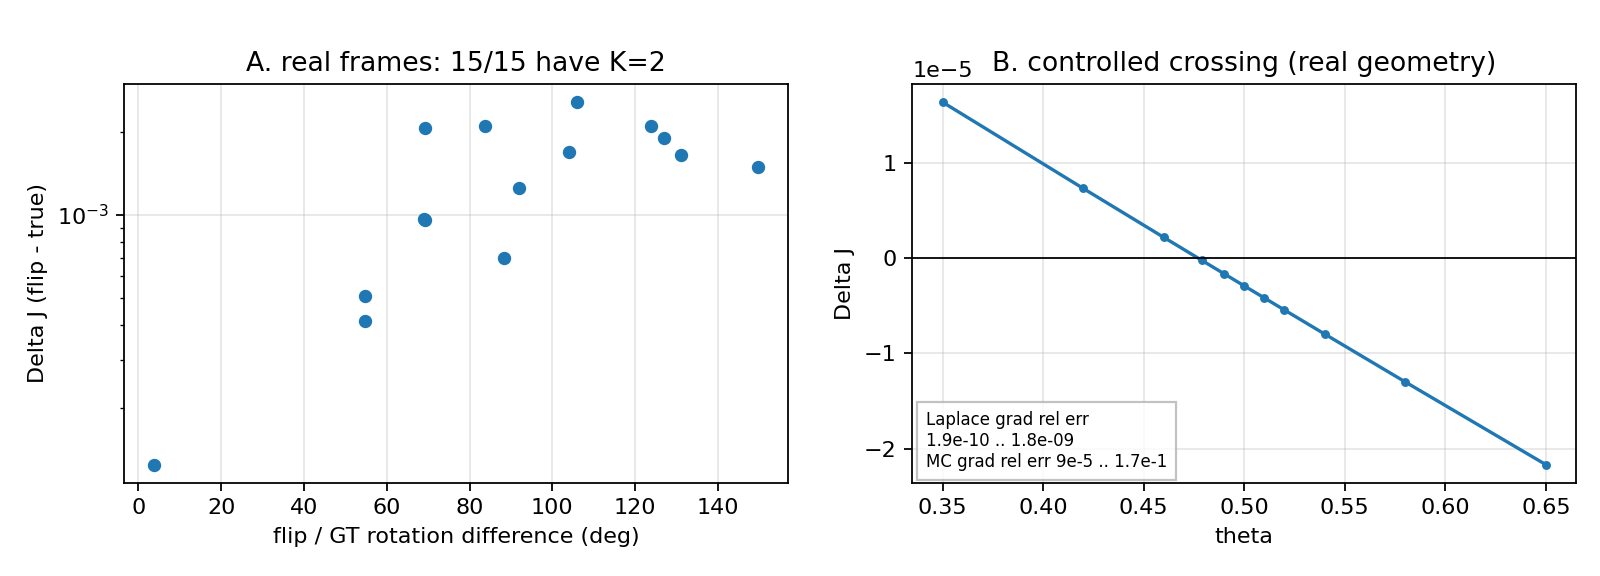
\includegraphics[width=\columnwidth]{two_mode.png}
\caption{The real two-mode cost. Left: for each of the 15 LINEMOD frames, the objective gap $\Delta J$ between the flip and the GT-like mode against the angle between the two modes; every frame has $K_{\rm phys}=2$, with $\Delta J\in[1.25\times10^{-4},2.56\times10^{-3}]$. Right: the controlled transverse crossing on real geometry (Part B), where the two labelled hypotheses are mixed as $J_\theta=(1-\theta)J_{\rm true}+\theta J_{\rm sym}$; $\Delta J$ changes sign near $\theta\approx0.475$. The inset reports the analytic Laplace gradient error against central FD ($1.9\times10^{-10}$--$1.8\times10^{-9}$) and the 400-sample MC error ($9\times10^{-5}$--$1.7\times10^{-1}$).}
\label{fig:twomode}
\end{figure}

Three points follow. First, the two-mode structure is reproducible: $K_{\rm phys}=2$ in 15/15 frames, with $\Delta J\in[1.25\times10^{-4},2.56\times10^{-3}]$, other-mode angles $3.8^\circ$--$149.6^\circ$ and $w({\rm other})=0.450$--$0.608$. Second, the GT-like mode is the lowest-$J$ physical mode in 14/15 frames, so the hard argmin is accurate: median rotation error $2.06^\circ$ $[1.47,3.49]$ and median ADD-S $3.7$ mm $[3.0,4.3]$, with one failure above $10^\circ$ (\texttt{000010/72}, $44.5^\circ$). Third, the Laplace posterior mean is not an accuracy win on these near-ties: median projected rotation error $44.24^\circ$ $[33.90,46.87]$, paired bias $+36.9^\circ$ $[+27.2,+44.9]$, median ADD-S $13.9$ mm $[10.3,20.2]$, i.e.\ roughly half the mass on the flip. The smallest Hessian determinant is $6.09\times10^{-3}$ (\texttt{000011/20}), so the flip mode is itself close to a fold.

\begin{table*}[t]
\centering
\caption{Aggregate pose error and ADD-S on the 15 real frames. Medians with 95\% percentile-bootstrap CIs over frames (1000 resamples). The paired bias is the mean per-frame difference against the hard argmin (95\% CI over frames); the median paired rotation bias is $+41.8^\circ$. ``Within $10^\circ$'' counts frames whose estimate is within $10^\circ$ of GT; for the posterior mean this is not a ``true mode'', since the mean need not be a mode.}
\label{tab:aggregate}
\scriptsize
\setlength{\tabcolsep}{3.5pt}
\begin{tabular}{@{}l l l l l l l@{}}
\toprule
method & rot med (deg) & ADD-S med (mm) & ADD med (mm) & rot bias (deg) & ADD-S bias (mm) & $\le10^\circ$ / true mode\\
\midrule
hard argmin & 2.06 [1.47, 3.49] & 3.7 [3.0, 4.3] & 5.9 [5.2, 11.1] & --- & --- & 14/15 true mode\\
Laplace (projected) & 44.24 [33.90, 46.87] & 13.9 [10.3, 20.2] & 38.1 [31.0, 41.5] & +36.9 [+27.2, +44.9] & +9.4 [+6.4, +12.6] & 0/15\\
MC (20 seeds) & 43.80 [33.90, 47.43] & 14.1 [10.3, 20.0] & 38.0 [31.0, 41.5] & +37.2 [+26.7, +45.0] & +9.4 [+6.4, +12.5] & 0/15\\
\bottomrule
\end{tabular}
\end{table*}

\begin{figure*}[t]
\centering
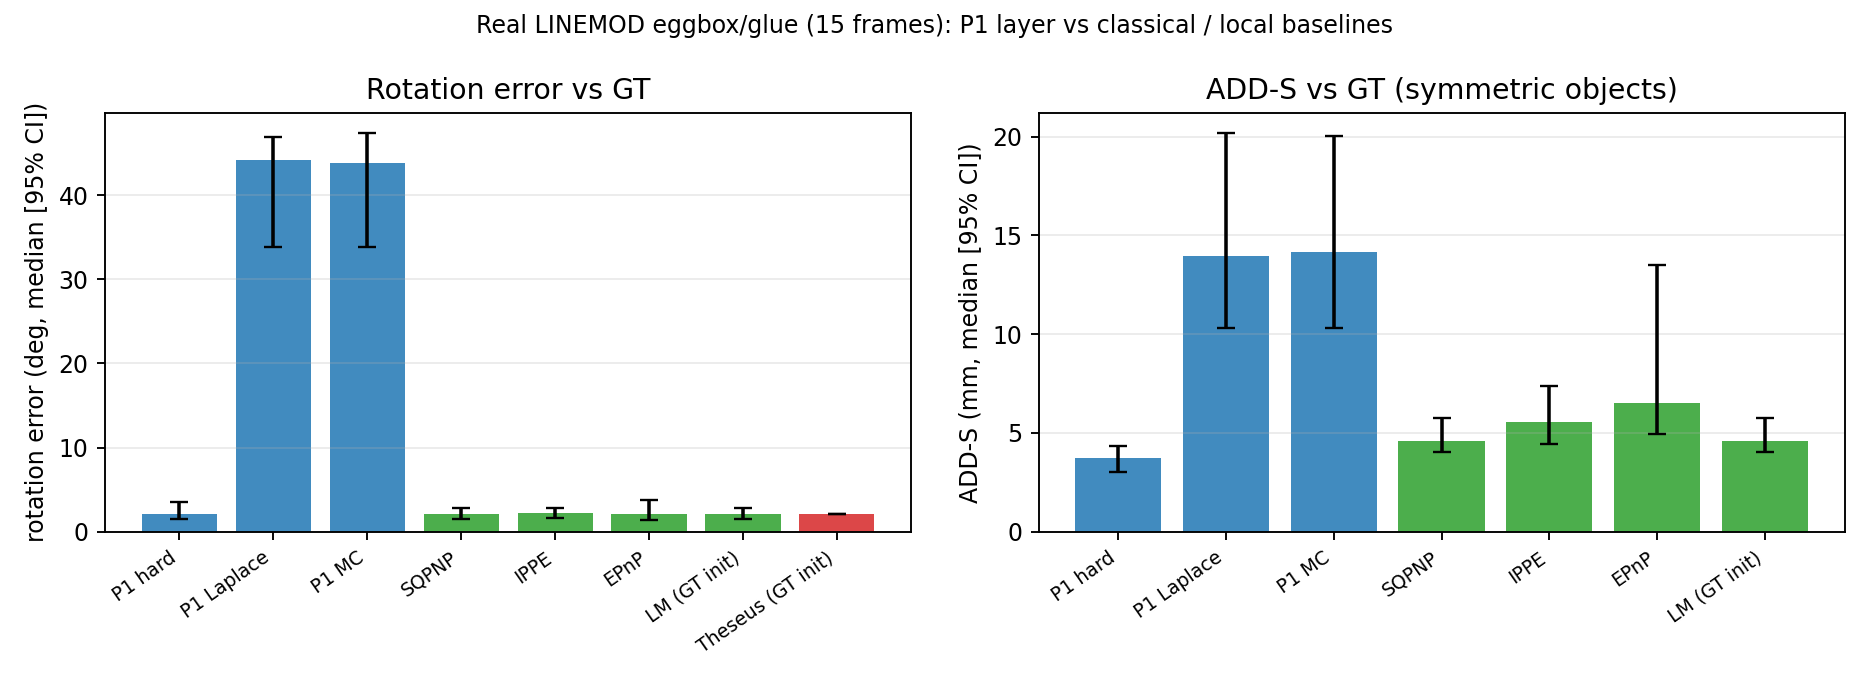
\includegraphics[width=\textwidth]{real_summary.png}
\caption{Real LINEMOD \texttt{eggbox}/\texttt{glue} results on the 15 frames, medians with 95\% bootstrap CIs. Left: rotation error against BOP ground truth for the P1 layer (hard argmin, projected Laplace mean, 20-seed MC) and for the forward/local references (SQPNP, IPPE, EPnP, local LM from GT init, Theseus from GT init). Right: ADD-S for the same methods (Theseus is not plotted). The hard argmin is at the classical-solver level; both posterior-mean estimates sit near $44^\circ$ because they average the two modes. Green bars are forward/local references; the red bar is a local solver started at ground truth and is not a deployable baseline.}
\label{fig:realsummary}
\end{figure*}

The 15-frame aggregates are in Table~\ref{tab:aggregate}. Means exceed medians for the hard argmin ($5.28^\circ$, $6.0$ mm) because of the single failure frame, while the Laplace means are $42.21^\circ$ and $15.5$ mm; translation medians are $6.2$ mm (hard) and $20.2$ mm (Laplace). MC estimates the same smooth mean ($0.23^\circ$ from the Laplace aggregate, within its seed-level CI) and inherits the bias, adding only seed noise (between-seed SD $1.011^\circ$).

\begin{table}[t]
\centering
\caption{Per-frame ADD-S (mm) and ADD reference (mm) on the 15 real frames. ADD-S is the primary object-space metric; ADD is same-index distance and is not invariant to the objects' $\sim180^\circ$ symmetry.}
\label{tab:perframe}
\scriptsize
\setlength{\tabcolsep}{2.5pt}
\begin{tabular}{@{}l r l l l l@{}}
\toprule
frame/img & obj & ADD-S hard & ADD-S Lap & ADD-S MC & ADD Lap (ref)\\
\midrule
000010/15 & 10 & 3.0 & 10.3 & 10.3 & 31.0\\
000010/18 & 10 & 4.3 & 12.2 & 12.3 & 37.6\\
000010/40 & 10 & 6.2 & 9.7 & 9.7 & 31.1\\
000010/60 & 10 & 3.0 & 13.9 & 14.1 & 40.7\\
000010/66 & 10 & 2.7 & 12.1 & 12.0 & 38.0\\
000010/72 & 10 & 12.5 & 8.4 & 8.4 & 22.3\\
000010/80 & 10 & 3.8 & 8.8 & 8.9 & 24.1\\
000010/90 & 10 & 3.1 & 8.5 & 8.4 & 23.3\\
000011/20 & 11 & 13.8 & 22.9 & 22.8 & 72.7\\
000011/24 & 11 & 2.8 & 20.2 & 20.0 & 40.5\\
000011/26 & 11 & 3.7 & 17.6 & 17.5 & 38.1\\
000011/32 & 11 & 3.1 & 19.0 & 19.0 & 41.5\\
000011/33 & 11 & 3.8 & 23.4 & 23.7 & 41.5\\
000011/40 & 11 & 2.2 & 16.8 & 16.7 & 44.7\\
000011/49 & 11 & 22.4 & 28.1 & 28.2 & 75.9\\
\bottomrule
\end{tabular}
\end{table}

Two per-frame readings matter. (i) On \texttt{000010/72} the hard argmin is the mode $44.5^\circ$ from GT while the GT-like mode is $3.8^\circ$ away but higher in $J$ by $1.25\times10^{-4}$; Laplace/MC land between the modes ($23.0^\circ$, $8.4$ mm) and are closer than the hard failure. That is a single-frame accident of the loss ranking, not evidence that the posterior mean is more accurate in general. (ii) ADD is $2$--$3\times$ ADD-S for the Laplace pose (median $38.1$ vs $13.9$ mm) because the glue object is long and thin and the $\sim180^\circ$ symmetry relabels it; this is why ADD-S, not ADD, is the reported metric.

\subsubsection{Classical forward solvers on the same correspondences}\label{sec:classical}

Table~\ref{tab:classical} runs cv2's EPnP, ITERATIVE, SQPNP and IPPE, plus a plain local GN/LM on the same bearing cost, on the bitwise-identical 15-frame correspondences (verified bitwise identical across the two studies; the GT-pose re-projection residual is $1.47$ px median, i.e.\ the $\sim1$ px nearest-vertex quantisation). These are forward solvers, not differentiable layers: the LM is a plain forward optimiser on the same cost, not BPnP, and no gradient claim is attached to any of them. IPPE is run on the RANSAC inliers projected onto the fitted plane (it requires exact coplanarity, planarity RMS $0.83$--$1.47$ mm); the other solvers use the raw inliers.

\begin{table*}[t]
\centering
\caption{Classical forward PnP baselines on the 15 real frames. Median with 95\% bootstrap CI over frames (2000 resamples). ``True mode'' counts solutions within $10^\circ$ of GT. SQPNP returns one solution in cv2 5.0.0 (documented for non-P3P/IPPE flags and observed on all 15 frames); IPPE returns two planar solutions, and the first (cheapest-reprojection) one is the GT-closer one on all 15 frames, so the oracle row would be identical to ``IPPE first''.}
\label{tab:classical}
\scriptsize
\setlength{\tabcolsep}{4pt}
\begin{tabular}{@{}l l l l@{}}
\toprule
method & rot median [CI] (deg) & ADD-S median [CI] (mm) & true mode\\
\midrule
EPnP & 2.05 [1.41, 3.71] & 6.5 [5.0, 13.5] & 12/15\\
ITERATIVE (homography init + LM) & 2.07 [1.60, 3.54] & 6.5 [5.7, 8.7] & 11/15\\
SQPNP (1 solution) & 2.04 [1.47, 2.77] & 4.6 [4.0, 5.8] & 15/15\\
IPPE (first, plane-projected) & 2.21 [1.68, 2.76] & 5.5 [4.4, 7.4] & 15/15\\
local LM, identity init & 106.01 [69.14, 179.82] & 40.7 [28.0, 1708.7] & 3/15\\
local LM, GT init & 2.06 [1.47, 2.77] & 4.6 [4.0, 5.8] & 15/15\\
local LM, flip init & 88.39 [69.08, 106.01] & 23.5 [16.9, 28.0] & 0/15\\
\bottomrule
\end{tabular}
\end{table*}

The ADD-S column here uses the 1000-query/1000-GT-vertex estimator, which carries a $+1.1$ mm discretisation floor relative to the dense-GT ADD-S of Table~\ref{tab:aggregate}; rotation error is the comparable column.

Three readings. (i) Forward point accuracy is at the classical level: SQPNP/EPnP/ITERATIVE medians are $2.04$--$2.07^\circ$ and IPPE is $2.21^\circ$, i.e.\ equal to the hard argmin's $2.06^\circ$ within frame noise; no classical solver comes near the Laplace mean's $44.2^\circ$. (ii) Single-solution solvers are confidently wrong on some frames: EPnP misses GT by more than $10^\circ$ on 3/15 and ITERATIVE on 4/15 (the fourth, \texttt{000011/20}, is $10.0^\circ$, at the threshold); on \texttt{000010/72} EPnP and ITERATIVE both return the planar flip at $44.3^\circ$/$44.0^\circ$ with a re-projection residual of $0.78$--$0.79$ px, and the flip even has lower bearing cost than the true-mode planar solution on the raw inliers. (iii) Without the $z>0$ physicality filter and multi-start, the local LM baseline fails from identity (3/15 true, 7/15 behind the camera; median $106^\circ$) and stays out of the true mode from the flip init (0/15); only the GT init recovers it. The physicality filter and enumeration therefore do real work on this cost.

\subsubsection{Theseus LM on the same cost}\label{sec:theseus}

Theseus 0.2.3 (\texttt{LevenbergMarquardt}, float64 CPU) minimises the same bearing cost \cite{pineda2022theseus}; its objective agrees with a numpy reference to $1.1\times10^{-13}$ and its analytic Jacobian matches central differences to $1.3\times10^{-10}$. It is a local optimiser: each call returns one pose, it has no notion of the enumerated mode set, it returns no posterior, and it applies no $z>0$ physicality filter.

\begin{table*}[t]
\centering
\caption{Theseus LM on the real bearing cost. ``True mode'' is within $10^\circ$ of GT. The random-init row pools 20 inits on each of the 15 frames (300 solves); the multistart row pools 8 inits on each of 5 representative frames (40 solves) and its median is over those 40 trial errors, not a best-of-8 aggregate.}
\label{tab:theseus}
\footnotesize
\setlength{\tabcolsep}{4pt}
\begin{tabular}{@{}l l l p{7.4cm}@{}}
\toprule
protocol & rot median (deg) & true mode & outcome breakdown\\
\midrule
GT init (15 frames) & 2.06 & 15/15 & recovers the nearest P1 mode (on \texttt{000010/72} that is the $3.8^\circ$ mode, not the global argmin)\\
identity init (15 frames) & 178.82 & 1/15 & 6 flip, 8 other; 8 behind the camera\\
20 random inits/frame (300 solves) & 123.91 & 100/300 (33.3\%) & 57 flip, 143 other, 134 non-physical\\
8 inits $\times$ 5 frames (40 solves) & 4.95 & 11/40 (27.5\%) & no aggregate posterior; per-trial errors\\
\bottomrule
\end{tabular}
\end{table*}

The GT-init row is local convergence, not a baseline win. From cold starts Theseus returns whichever basin the descent enters---often the flip mode or a behind-camera stationary point of the unconstrained cost, exactly the solutions the layer's enumeration rejects. It is the natural no-enumeration reference on this near-tied cost; local optimisation does not replace mode enumeration.

\subsubsection{Controlled transverse crossing on real geometry}\label{sec:partb}

Part B removes the shared-translation failure of the old construction: each of two labelled hypotheses eliminates its \textbf{own} translation, and the costs are mixed as $J_\theta=(1-\theta)J_{\rm true}+\theta J_{\rm sym}$. On the real frame \texttt{000010/15} the measured tie is at $\theta^\star\approx0.475$ (the construction is designed to tie at $0.5$, but resampling makes the two labelled costs not exactly symmetric); $\Delta J$ changes sign between $\theta=0.46$ and $0.479$, so the crossing is transverse, and the two minima stay within $\sim2^\circ$ of their labelled poses.

\begin{table}[t]
\centering
\caption{Controlled transverse crossing on real geometry (Part B, excerpt). \emph{grad rel} is the analytic Laplace gradient against central FD of the layer output; MC is mode-level with 400 samples.}
\label{tab:partb}
\scriptsize
\setlength{\tabcolsep}{2.5pt}
\begin{tabular}{@{}l l l l l l@{}}
\toprule
$\theta$ & $\Delta J$ & $w(A)$ & Laplace grad rel & MC grad rel & $\|d\phi\|$\\
\midrule
0.3500 & +1.64e-05 & 0.50031 & 2.59e-10 & 9.51e-03 & 1.129e-02\\
0.4600 & +2.20e-06 & 0.50004 & 8.61e-10 & 8.94e-05 & 1.123e-02\\
0.4790 & -2.22e-07 & 0.50000 & 7.82e-10 & 1.68e-01 & 1.122e-02\\
0.5000 & -2.89e-06 & 0.49995 & 1.76e-09 & 5.09e-02 & 1.121e-02\\
0.6500 & -2.17e-05 & 0.49960 & 4.03e-10 & 1.10e-02 & 1.112e-02\\
\bottomrule
\end{tabular}
\end{table}

Across the 11 rows the Laplace gradient agrees with central FD to $1.9\times10^{-10}$--$1.8\times10^{-9}$, while the 400-sample mode-level MC error is $8.9\times10^{-5}$--$1.7\times10^{-1}$; the hard argmin has a jump at the tie and its FD is undefined there, so no hard gradient is reported. This is a correctness result for the closed-form backward pass on a real cost; the ADD-S proxy belongs to Part A.

\subsection{Runtime and batching}\label{sec:compute}

\textbf{CPU only.} All reported runs are CPU-only single-process jobs. The SDP runs use cvxpy 1.9.3/SCS ($\varepsilon=10^{-9}$, \texttt{max\_iters=200000}), cvxpy 1.7.5/SCS for the comparison, and SCS with $\varepsilon=10^{-11}$, \texttt{max\_iters=10\textasciicircum 6} for the 6-point check. The real-data and root-count runs are short CPU jobs: the pose-error/ADD-S run takes $\approx10$ s, the classical baselines $3.0$ s, the Theseus comparison $9.5$ s, and the root count $\approx30$ s for four instances.

\textbf{Timing.} From 20 repetitions, a full synthetic layer call at $\theta=0$ takes 61.9 ms median (p95 62.1): mode enumeration is 88\%, the $K$ implicit $3\times3$ solves 1.6\%, and the analytic backward pass (weight gradient and mixing) 0.1\%. At $\theta=-0.1$ the whole call is 17.7 ms. The LINEMOD runs report 24.2--265.9 ms per frame forward and 33.1--42.6 ms per $\theta$ including FD for the transverse crossing.

\textbf{Batching.} A true batched multi-start Newton is only $1.30\times$ faster than the loop at batch size 64 (59.9 versus 46.2 samples/s), $0.78\times$ at 8, and $0.46\times$ at 1: convergence heterogeneity and the per-instance classify loop dominate, so a GPU or custom kernel is needed for a real throughput win. Mode enumeration is the bottleneck, not the $3\times3$ solves.
